\documentclass[sigconf]{acmart}
%%
%% \BibTeX command to typeset BibTeX logo in the docs
\AtBeginDocument{%
  \providecommand\BibTeX{{%
    Bib\TeX}}}

%% Rights management information.  This information is sent to you
%% when you complete the rights form.  These commands have SAMPLE
%% values in them; it is your responsibility as an author to replace
%% the commands and values with those provided to you when you
%% complete the rights form.
\setcopyright{acmlicensed}
\copyrightyear{2026}
\acmYear{2026}
\acmDOI{XXXXXXX.XXXXXXX}
%% These commands are for a PROCEEDINGS abstract or paper.
\acmConference[KDD-UC '26]{ACM SIGKDD Undergraduate Consortium}{August 09--13}{Jeju, Korea}
%%
%%  Uncomment \acmBooktitle if the title of the proceedings is different
%%  from ``Proceedings of ...''!
%%
%%\acmBooktitle{Woodstock '18: ACM Symposium on Neural Gaze Detection,
%%  June 03--05, 2018, Woodstock, NY}
\acmISBN{978-1-4503-XXXX-X/2026/08}


%%
%% Submission ID.
%% Use this when submitting an article to a sponsored event. You'll
%% receive a unique submission ID from the organizers
%% of the event, and this ID should be used as the parameter to this command.
%%\acmSubmissionID{123-A56-BU3}

%%
%% For managing citations, it is recommended to use bibliography
%% files in BibTeX format.
%%
%% You can then either use BibTeX with the ACM-Reference-Format style,
%% or BibLaTeX with the acmnumeric or acmauthoryear sytles, that include
%% support for advanced citation of software artefact from the
%% biblatex-software package, also separately available on CTAN.
%%
%% Look at the sample-*-biblatex.tex files for templates showcasing
%% the biblatex styles.
%%

%%
%% The majority of ACM publications use numbered citations and
%% references.  The command \citestyle{authoryear} switches to the
%% "author year" style.
%%
%% If you are preparing content for an event
%% sponsored by ACM SIGGRAPH, you must use the "author year" style of
%% citations and references.
%% Uncommenting
%% the next command will enable that style.
%%\citestyle{acmauthoryear}


%%
%% end of the preamble, start of the body of the document source.
\begin{document}

%%
%% The "title" command has an optional parameter,
%% allowing the author to define a "short title" to be used in page headers.
\title{Decomposition vs Augmentation: Isolating the Impact of Multi-Agent Architectures in Entity Resolution}

%%
%% The "author" command and its associated commands are used to define
%% the authors and their affiliations.
%% Of note is the shared affiliation of the first two authors, and the
%% "authornote" and "authornotemark" commands
%% used to denote shared contribution to the research.
\author{Zachary Zeng}
% \authornote{Both authors contributed equally to this research.}
\email{zengz1@ufl.edu}
% \orcid{1234-5678-9012}}
% \authornotemark[1]
\affiliation{%
  \institution{University of Florida}
  \city{Gainesville}
  \state{Florida}
  \country{USA}
}

%%
%% By default, the full list of authors will be used in the page
%% headers. Often, this list is too long, and will overlap
%% other information printed in the page headers. This command allows
%% the author to define a more concise list
%% of authors' names for this purpose.
\renewcommand{\shortauthors}{Zeng}

%%
%% The abstract is a short summary of the work to be presented in the
%% article.
\begin{abstract}
Recent work reports that multi-agent large language model (LLM) systems outperform single-LLM pipelines on entity resolution (ER), but these systems typically bundle agent decomposition with retrieval-augmented generation or other external knowledge, conflating two design choices. This paper separates them with a three-way comparison on Abt-Buy: a Magellan-style random-forest baseline, a single \texttt{gpt-oss-120b} pipeline, and a multi-agent \texttt{gpt-oss-120b} pipeline whose syntactic and semantic agents share only local, computable tools under an orchestrator, without external retrieval or task-specific context at inference. Across five runs on one fixed 1,916-pair labeled test split, the single-LLM pipeline attains slightly higher mean $F_1$ than the multi-agent pipeline ($0.9065 \pm 0.0039$ vs.\ $0.8973 \pm 0.0048$; $\Delta F_1 = +0.0092$, exact permutation test $p = 0.0238$), while the two agree on $98.8\%$ of decisions ($\kappa = 0.9426 \pm 0.0075$). The multi-agent pipeline consumes $8.7\times$ more tokens and runs $6.6\times$ longer, trading recall ($0.920$ vs.\ $0.960$) for precision ($0.875$ vs.\ $0.859$). On this benchmark, decomposition without knowledge augmentation acts as a precision-recall adjustment rather than an accuracy gain.
\end{abstract}


%%
%% The code below is generated by the tool at http://dl.acm.org/ccs.cfm.
%% Please copy and paste the code instead of the example below.
%%
\begin{CCSXML}
<ccs2012>
<concept>
<concept_id>10002951.10003317.10003347.10003352</concept_id>
<concept_desc>Information systems~Information extraction</concept_desc>
<concept_significance>500</concept_significance>
</concept>
<concept>
<concept_id>10010147.10010178.10010187</concept_id>
<concept_desc>Computing methodologies~Knowledge representation and reasoning</concept_desc>
<concept_significance>300</concept_significance>
</concept>
<concept>
<concept_id>10010405</concept_id>
<concept_desc>Applied computing</concept_desc>
<concept_significance>100</concept_significance>
</concept>
<concept>
<concept_id>10010147.10010257.10010293</concept_id>
<concept_desc>Computing methodologies~Machine learning approaches</concept_desc>
<concept_significance>100</concept_significance>
</concept>
</ccs2012>
\end{CCSXML}

\ccsdesc[500]{Information systems~Information extraction}
\ccsdesc[300]{Computing methodologies~Knowledge representation and reasoning}
\ccsdesc[100]{Applied computing}
\ccsdesc[100]{Computing methodologies~Machine learning approaches}

%%
%% Keywords. The author(s) should pick words that accurately describe
%% the work being presented. Separate the keywords with commas.
\keywords{Entity Resolution, Large Language Models, Multi-Agent Systems, Knowledge Augmentation, Retrieval-Augmented Generation, Agent Decomposition, Zero-shot Classification, Product Matching}

%% A "teaser" image appears between the author and affiliation
%% information and the body of the document, and typically spans the
%% page.
% \begin{teaserfigure}
%   \includegraphics[width=\textwidth]{sampleteaser}
%   \caption{Seattle Mariners at Spring Training, 2010.}
%   \Description{Enjoying the baseball game from the third-base
%   seats. Ichiro Suzuki preparing to bat.}
%   \label{fig:teaser}
% \end{teaserfigure}

\received{1 May 2026}
\received[revised]{31 July 2026}
\received[accepted]{1 September 2026}

%%
%% This command processes the author and affiliation and title
%% information and builds the first part of the formatted document.
\maketitle

\section{Introduction}

Entity resolution (ER), or record linkage, is the task of identifying which records across one or more datasets refer to the same real-world entity~\cite{binette2022almost}.
It is a critical step in data cleaning whose precision directly bounds downstream analysis quality, with applications from census deduplication to academic publication disambiguation~\cite{christophides2020overview}.
Large language models (LLMs) have recently emerged as a third option alongside rule-based systems and feature-engineered classifiers, leveraging pre-trained world knowledge to assess entity similarity through natural-language reasoning rather than labeled training data and hand-crafted features~\cite{wang2025match, zhang2025deep}.
This expressiveness, however, comes at a real cost: each pair requires an API call that incurs token-based charges and network latency, so the practical case for LLM-based ER hinges on whether the accuracy gains justify the overhead~\cite{li2024booster, nananukul2024cost}.

A second wave of LLM-based ER work has moved beyond monolithic prompting toward multi-agent architectures, in which specialized agents analyze different aspects of a candidate pair and a coordinator produces the final verdict.
Such systems report accuracy gains over single-LLM baselines for ER in Althaf et al.~\cite{althaf2025multi}, and for the adjacent task of zero-shot named-entity recognition in CMAS~\cite{wang2025cooperative}.
However, they typically bundle agent decomposition with retrieval-augmented generation (RAG), self-annotated training data, or other forms of external knowledge.
As a result, the reported gains conflate two distinct design choices: \emph{decomposing} the reasoning across agents, and \emph{augmenting} the agents with information beyond the pair itself.
It is not clear whether the multi-agent architecture alone helps ER, or whether the accuracy gains are attributable to the augmentation component and would disappear if the agents were given only the pair and local tools.

This paper isolates that question with a controlled three-way comparison on the Abt-Buy product-catalog benchmark.
I evaluated a Magellan-style random-forest baseline~\cite{konda2016magellan}, a single \texttt{gpt-oss-120b} model baseline, and a multi-agent \texttt{gpt-oss-120b} pipeline on the same fixed 1,916-pair labeled test split, with identical metrics.
The multi-agent pipeline does not include retrieval or external knowledge.
Instead, it features a syntactic agent equipped with string-similarity tools (a Ratcliff-Obershelp sequence-matching score, word-token Jaccard, and BM25) and a semantic agent equipped with sentence-embedding cosine similarity and a price comparator.
These two agents are coordinated by an orchestrator that merges their verdicts into a final decision.
Holding the base model fixed and withholding retrieval from both LLM configurations removes the knowledge-augmentation confound; the multi-agent arm still changes the prompts, call count, tools, and aggregation step at once, so the two LLM arms are read as bundled configurations rather than as a marginal effect of decomposition.

This paper makes three contributions.
First, it provides a three-way benchmark between a Magellan-style Random Forest, a single-LLM pipeline, and a multi-agent LLM pipeline on the Abt-Buy benchmark over one fixed labeled test split, with no retrieval or task-specific context given to the LLM pipelines at inference.
Second, it reports a cost-efficiency evaluation that includes precision, recall, $F_1$, token consumption, and end-to-end runtime averaged over five separate executions per pipeline, exposing the cost-performance trade-off for practitioners.
Third, it presents an error analysis of the pairs in which the two LLM pipelines disagree, categorizing their false positives and false negatives to describe complementary error profiles that accompany the architectural differences.

The results show a small but consistent single-LLM advantage in mean $F_1$ ($0.9065 \pm 0.0039$ vs.\ $0.8973 \pm 0.0048$; exact permutation $p = 0.0238$), with the two configurations agreeing on $98.8\%$ of decisions.
The multi-agent pipeline consumes $8.7\times$ more tokens and runs $6.6\times$ longer while occupying a different point on the precision-recall plane, trading aggressive matches on sparse listings for stricter rejection of color and finish variants.


\section{Related Work}
\label{sec:related}

\subsection{Entity Resolution Background}
Entity resolution has been studied for decades under several names (record linkage, entity matching, deduplication), and modern end-to-end pipelines decompose the task into \textit{blocking}, \textit{matching}, and \textit{clustering}~\cite{binette2022almost, christophides2020overview}; this paper focuses on the matching stage, evaluating every matcher on one fixed labeled pair set.
Early ER relied on Fellegi-Sunter-style probabilistic rules with hand-tuned similarity thresholds~\cite{hussein2025llm}; modern supervised approaches such as Magellan~\cite{konda2016magellan} (this paper's baseline) automatically generate a dense feature vector of attribute-level similarities (edit distance, Jaccard, Monge-Elkan, TF-IDF cosine) and train a standard classifier on labeled pairs.
Deep-learning approaches like DITTO~\cite{li2020deep} further improved matching by fine-tuning a pre-trained language model on labeled pairs, but they still require task-specific labeled data and per-dataset fine-tuning, motivating the shift toward prompting-based methods.

\subsection{LLM-Based Entity Resolution}
LLM-based ER lets a pre-trained model decide whether two records describe the same entity directly from a natural-language prompt, without task-specific training~\cite{hussein2025llm}.
Wang et al.~\cite{wang2025match} identified three prompting strategies: \textit{match} (one pair at a time), \textit{compare} (one record against many), and \textit{select} (pick the best match from a set); this paper's single-LLM baseline uses the \textit{match} strategy as the most direct comparison to traditional pair-classifiers.
BoostER complements this design by using the LLM as a selective verifier on top of a cheaper base matcher, reducing the number of LLM calls per dataset~\cite{li2024booster}, and prompt-engineering work has further explored single-attribute prompts and caching to contain token cost~\cite{nananukul2024cost}.
Importantly, recent cross-dataset evaluation shows that fine-tuned small models can rival frontier closed models on entity matching~\cite{zhang2025deep}, which justifies the use of a medium-sized open model, \texttt{gpt-oss-120b}, in this study.

\subsection{Multi-Agent LLM Systems and the Knowledge-Augmentation Confound}
A new paradigm of LLM work uses multi-agent architectures, where specialized agents analyze different aspects of an input and an orchestrator coordinates their verdicts~\cite{guo2024large}.
For ER, Althaf et al.~\cite{althaf2025multi} report gains over single-LLM baselines using a layered framework whose agents retrieve context from an indexed knowledge store via a RAG component. Their results show that gains are positive both with and without that RAG layer (single-LLM $F_1$ 86.4, multi-agent without retrieval 88.5, with RAG 93.4), so their own ablation is evidence \emph{against} attributing the whole improvement to retrieval.
CMAS~\cite{wang2025cooperative} pairs decomposition with self-annotated pseudo-labels and retrieved few-shot demonstrations, but it is evaluated on zero-shot named-entity recognition benchmarks rather than on entity resolution.
In every reported gain, however, decomposition is coupled with some added source of information beyond the input pair, so the existing literature cannot tell whether the improvements stem from decomposition or from the accompanying knowledge augmentation.
This study targets that confound directly: agents have access only to local, computable tools over the pair itself, isolating what decomposition alone contributes to performance and efficiency.


\section{Method}
\label{sec:method}

\subsection{Data and Blocking}
I use the Abt-Buy product dataset from HuggingFace\footnote{\url{https://huggingface.co/datasets/matchbench/Abt-Buy}}: 1,081 listings from Abt.com and 1,092 from Buy.com, paired into 9,575 labeled candidate pairs with 1,028 verified true matches.
Each record carries a name, description, and price (with some missing values), and the dataset is presplit into train (5,743 pairs, 616 positive), validation, and test (each 1,916 pairs, 206 positive) splits, yielding a 10.8\% positive-class rate on the test split used for all final metrics.

To reduce the $1{,}081 \times 1{,}092 = 1{,}180{,}452$-pair Cartesian product, I apply TF-IDF cosine-similarity blocking on product names with character 2- and 3-gram features and a similarity threshold of $0.2$, retaining 16,629 candidate pairs that contain 100\% of true matches.

The blocker characterizes a deployment configuration and is \emph{not} on the evaluated path: every reported metric is computed over the dataset's own 1,916-pair labeled test split, passed directly to each matcher, so all three pipelines see an identical pair set and observed differences are attributable to the matcher.

\subsection{Magellan Pipeline}
The traditional ML baseline is \emph{Magellan-style} rather than a run of Magellan itself: it follows the approach of~\cite{konda2016magellan}, using a Random Forest classifier over manually engineered features.
Because the original \texttt{py\_entitymatching} library was incompatible with my Python 3.12 environment, I reimplemented the feature set from Magellan's source using \texttt{scikit-learn} and \texttt{jellyfish} to approximate its auto-generated features. Results for this baseline should therefore be read as a faithful manual adaptation, not as the Magellan library's own output.
Each pair is encoded as 14 features: 8 string similarities over names (3-gram and word-token Jaccard, TF-IDF cosine, Monge-Elkan with Jaro-Winkler, raw and normalized Levenshtein, Needleman-Wunsch and Smith-Waterman alignment), 2 over descriptions (3-gram Jaccard, TF-IDF cosine), and 4 over prices.
The classifier was trained on the predefined training split, with hyperparameters and the decision threshold tuned by \texttt{GridSearchCV} over a \texttt{PredefinedSplit} on the validation set to maximize $F_1$ (full grid in the released code).

\subsection{Single-LLM Pipeline}
The single-LLM baseline utilizes the \texttt{gpt-oss-120b} model with a direct prompt-response mechanism.
Each pair is sent with a system prompt that directs the model to weigh name variations, matching specifications such as model numbers, price compatibility, and description overlap, and to reply with a JSON object holding a binary verdict, a confidence in $[0.0, 1.0]$, and a brief rationale (full prompt in Appendix~\ref{sec:prompts}).
Pairs are processed sequentially at temperature 0, and every response is cached locally for post-hoc analysis.

\subsection{Multi-Agent LLM Pipeline}
The multi-agent LLM architecture decomposes entity resolution into specialized lenses handled by two reviewer agents that are coordinated by a central orchestrator.
All agents and the orchestrator use \texttt{gpt-oss-120b}, and each agent has a fixed tool-set.

The syntactic agent focuses on string-level similarity and is given three Model Context Protocol (MCP) tools: a normalized sequence-matching dissimilarity over product names, word-token Jaccard similarity over product names, and a symmetric BM25 relevance score normalized to $[0, 1]$.

The sequence-matching tool returns $1 - r$, where $r$ is Python's \texttt{difflib.SequenceMatcher} ratio (a Ratcliff-Obershelp measure), so 0.0 denotes identical names; full tool definitions, including the BM25 corpus construction and normalization, are given in Appendix~\ref{app:repro}.

The semantic agent focuses on deeper semantic analysis and is given two MCP tools that it is also instructed to call before deciding: a price comparator that returns the price ratio, absolute difference, and a similarity flag (ratio $\geq 0.8$) over the two parsed prices, and an embedding cosine similarity computed between \texttt{all-MiniLM-L6-v2} sentence-transformer embeddings of the product names.

Tools are served via FastMCP over a stdio transport, running as a subprocess that communicates with the agents through standard input/output, which separates tool execution from LLM inference.
The orchestrator receives the original product pair alongside both agents' structured responses (verdict, confidence, and reasoning) and is prompted to review and produce a final decision.
Every component (agent or orchestrator) returns a structured JSON response of the form \{verdict, confidence, reasoning\}, and the orchestrator's verdict serves as the final binary match decision for each
candidate pair.
Figure~\ref{fig:arch} illustrates the complete system architecture.

\begin{figure}[t]
  \centering
  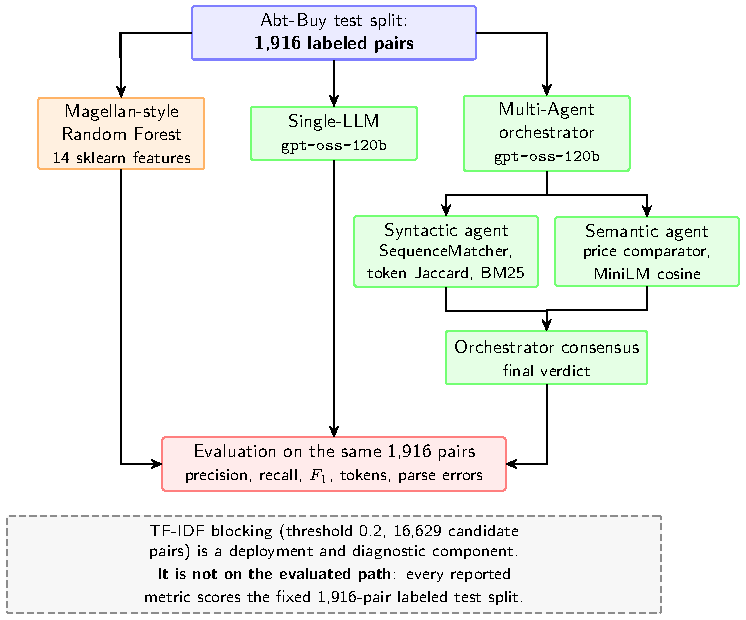
\includegraphics[width=\columnwidth]{figures/architecture.pdf}
  \Description{Block diagram. The fixed 1,916-pair labeled Abt-Buy test split feeds three matchers in parallel: a Magellan-style Random Forest with 14 sklearn features, a Single-LLM pipeline, and a Multi-Agent orchestrator. The orchestrator dispatches each pair to a syntactic agent (SequenceMatcher, token Jaccard, BM25) and a semantic agent (price comparator, MiniLM cosine), whose verdicts return to an orchestrator consensus step. All three matchers feed one shared evaluation harness. A separate detached box notes that TF-IDF blocking, which produces 16,629 candidate pairs, is a deployment and diagnostic component that is not on the evaluated path.}
  \caption{System architecture. The fixed 1,916-pair labeled test split is passed directly to all three matchers, which are scored by one shared harness. The multi-agent pipeline dispatches each pair to a syntactic and a semantic agent equipped with MCP tools, after which the orchestrator produces the consensus verdict. TF-IDF blocking is shown detached because it characterizes a deployment configuration and did not filter the evaluated pairs.}
  \label{fig:arch}
\end{figure}

\subsection{Evaluation Pipeline}
All three pipelines share one evaluation harness over the fixed 1,916-pair test split.
Each emits a verdict, a confidence, and a parse-error flag (failed JSON parses are recorded, not dropped); tokens are summed across LLM calls per pair, and are zero for Magellan since its inference is local.
Each LLM run uses an isolated cache, and Magellan's run-to-run variability comes solely from the Random Forest \texttt{random\_state}.


\section{Experiments}
\label{sec:experiments}

\subsection{Evaluation Metrics}
The primary metric is $F_1$, which balances false positives and false negatives without favoring either precision or recall. For the LLM pipelines, I additionally track total tokens consumed and end-to-end runtime, capturing the practical overhead of LLM-based ER relative to traditional ML.
The multi-agent pipeline is compared on $F_1$ against both the Magellan and single-LLM baselines, on runtime against both, and on tokens against the single-LLM, to determine whether any performance delta justifies the increased computational cost.

To quantify agreement between the two LLM pipelines beyond chance,
I compute Cohen's $\kappa$ over all $5 \times 5 = 25$ pairings of a single-LLM run with a multi-agent run and report the mean and sample standard deviation across those pairings; the configurations were executed independently, so no run-index correspondence exists and any single index-aligned pairing would be arbitrary.

To assess whether the residual $F_1$ gap reflects more than run-to-run noise, the unit of inference is the execution, not the pair: I compare the five run-level $F_1$ values per configuration with an exact, two-sided, unpaired, studentized permutation test over all $\binom{10}{5} = 252$ assignments, which is exact under the null that the ten executions are exchangeable between configurations.

\subsection{Experiment Setup}
All experiments ran on an Apple M4 Pro (24 GB RAM, macOS) with Python 3.12 and \texttt{uv} for dependency management. LLM calls used \texttt{gpt-oss-120b} via the OpenAI Python SDK at temperature 0, issued sequentially for comparable runtime measurements. Each pipeline was evaluated on the same 1,916 test-split pairs across 5 separate executions (Magellan variability comes from the Random Forest \texttt{random\_state}; LLM variability from residual API non-determinism at temperature 0), and I report the mean and standard deviation for all metrics.

\subsection{Pipeline Performance Comparison}

Table~\ref{tab:main-results} presents the aggregate performance of all three pipelines averaged across five separate executions each, treated as independent and exchangeable for inference.
The two LLM pipelines reach closely comparable $F_1$ values: the single-LLM baseline achieves $0.9065 \pm 0.0039$ and the multi-agent pipeline achieves $0.8973 \pm 0.0048$.
The exact execution-level permutation test resolves this small gap in the single-LLM's favor: $\Delta F_1 = \text{single-LLM} - \text{multi-agent} = +0.0092$, with 6 of the 252 allocations at least as extreme as the observed studentized statistic ($T = 3.355$), giving $p = 6/252 = 0.0238$.
The supported claim is narrow: across repeated executions on this fixed Abt-Buy test set, the single-LLM configuration had higher mean $F_1$ than the multi-agent configuration.
The entity-cluster sensitivity range, $[-0.0226, +0.0443]$, includes zero: with record- and execution-level uncertainty admitted jointly, the benchmark is compatible with either ordering, so the ranking is a statement about these executions on these pairs.
Both LLM pipelines substantially outperform the Magellan-style Random Forest baseline ($F_1 = 0.6066 \pm 0.0161$, roughly 30 points lower); the per-error breakdown is in \S\ref{sec:error-analysis}.

\begin{table}[h]
  \centering
  \caption{Aggregate performance across five runs (mean $\pm$ sample standard deviation, $n-1$) on the fixed 1,916-pair labeled test split. Accuracy and token metrics derive from the released prediction caches; runtime comes from separate sequential timing executions. The best result in each row is shown in bold; for cost metrics, lower is better.}
  \label{tab:main-results}
  \small
  \begin{tabular}{lccc}
    \toprule
    \textbf{Metric} & \textbf{Magellan} & \textbf{Single-LLM} & \textbf{Multi-Agent} \\
    \midrule
    Precision     & $0.6876 \pm 0.0186$ & $0.8585 \pm 0.0058$  & $\mathbf{0.8754 \pm 0.0075}$  \\
    Recall        & $0.5427 \pm 0.0147$ & $\mathbf{0.9602 \pm 0.0022}$  & $0.9204 \pm 0.0106$  \\
    $F_1$         & $0.6066 \pm 0.0161$ & $\mathbf{0.9065 \pm 0.0039}$  & $0.8973 \pm 0.0048$  \\
    Runtime (s)   & $\mathbf{10.0 \pm 0.1}$      & $2{,}538.9 \pm 340.4$ & $16{,}878.5 \pm 285.1$ \\
    Total tokens  & $\mathbf{0}$                 & $1{,}257{,}041 \pm 627$ & $10{,}959{,}451 \pm 24{,}899$ \\
    Tokens / pair & $\mathbf{0}$                 & $656.1 \pm 0.3$       & $5{,}720.0 \pm 13.0$ \\
    \bottomrule
  \end{tabular}
\end{table}

Magellan's cost is negligible: about 10 seconds per run and zero tokens, since inference is entirely local.
The single-LLM baseline takes about 42 minutes per run and the multi-agent pipeline about 281 minutes ($6.6\times$ longer), while also consuming $8.7\times$ more tokens per pair (5,720 vs.\ 656).
The multi-agent pipeline therefore costs substantially more in time and tokens without an accuracy gain, making the single-LLM the more cost-efficient LLM option on this benchmark.

Despite this cost asymmetry, the two LLM pipelines are closely aligned in their individual decisions: over all 25 pairings of a single-LLM run with a multi-agent run, Cohen's $\kappa$ averages $0.9426 \pm 0.0075$ and decision agreement averages $98.8 \pm 0.15\%$, indicating that multi-agent decomposition reaches largely the same verdicts as the single-LLM at a higher cost.

\subsection{Precision-Recall Trade-off}
\label{sec:pr}
Although the two LLM pipelines are tied in $F_1$, they occupy different points on the precision-recall curve, and the direction of the trade-off is informative.
Across the five runs, the multi-agent pipeline achieves higher precision ($0.875 \pm 0.008$ vs.\ $0.859 \pm 0.006$) at the cost of lower recall ($0.920 \pm 0.011$ vs.\ $0.960 \pm 0.002$).
In absolute terms on one illustrative run (Run~1, released as \texttt{eval\_run\_0}, also used for the error analysis below), the single-LLM baseline produces 33 false positives and 8 false negatives, while the multi-agent pipeline produces 26 false positives and 14 false negatives. Run~1 is the multi-agent pipeline's \emph{best} run, so it illustrates the error profiles rather than representing the average case.
The multi-agent pipeline is more conservative: it finds fewer positives, but the matches it declares are more consistently correct.
Sweeping the decision threshold over each pipeline's reported confidence (Figure~\ref{fig:pr-curves}) shows that this rebalancing persists beyond the default operating point.
At the threshold-optimized cut-offs, the multi-agent pipeline reaches its best $F_1 = 0.916$ at $\tau = 0.76$ while the single-LLM reaches $F_1 = 0.909$ at $\tau = 0.79$.
The supported finding is qualitative: the two configurations stay close across the threshold range.

\begin{figure}[t]
  \centering
  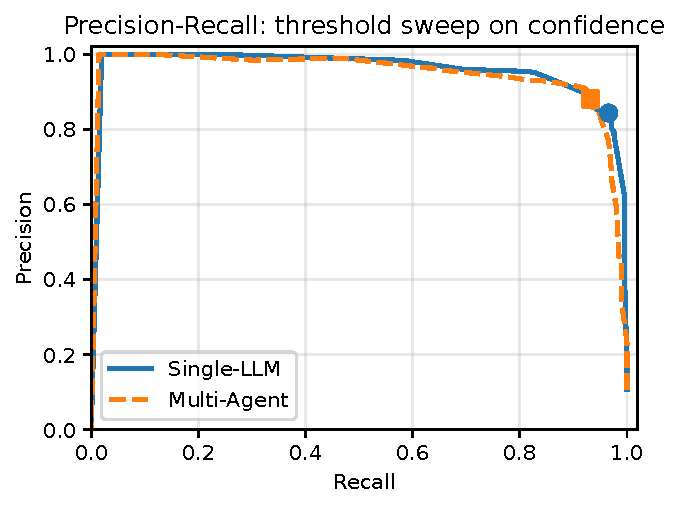
\includegraphics[width=\columnwidth]{figures/pr_curves.pdf}
  \Description{Two precision-recall curves with similar area; the multi-agent curve sits slightly above in the high-precision region. Default operating points at tau equals 0.5 are marked.}
  \caption{Precision-Recall curves for the two LLM pipelines on Run~1, obtained by sweeping the decision threshold $\tau \in [0,1]$ over each pipeline's reported confidence. The reported optima are 0.916 (multi-agent, $\tau = 0.76$) and 0.909 (single-LLM, $\tau = 0.79$). Both pipelines reach 0.906 at the default $\tau = 0.5$, which is the operating point used everywhere else in this paper.}
  \label{fig:pr-curves}
\end{figure}

\subsection{Error Analysis}
\label{sec:error-analysis}

False positives and false negatives from one illustrative run (Run~1) are assigned to categories by deterministic keyword and attribute rules over the product names, descriptions, and each model's reasoning field, in the released \texttt{analyze\_final\_results.py}; results appear in Table~\ref{tab:error-cats}.
The assignment is heuristic and reproducible rather than manually adjudicated.
These categories describe patterns in the models' rationales and predictions, not verified mechanisms: self-explanations need not faithfully reflect the computation behind a verdict, and across three LLMs and ten ER datasets Teofili et al.~\cite{teofili2026trust} find them unstable and weakly faithful.

\begin{table}[h]
  \centering
  \caption{False positive and false negative error categories for the two LLM pipelines on one illustrative run (Run~1). Categories are assigned by reproducible keyword and attribute rules over the models' generated rationales; they are descriptive, not verified mechanisms. The lower (better) pipeline total is shown in bold; for error counts lower is better.}
  \label{tab:error-cats}
  \small
  \begin{tabular}{lcc}
    \toprule
     & \textbf{Single-LLM} & \textbf{Multi-Agent} \\
    \midrule
    \multicolumn{3}{l}{\textit{False positives}} \\
    \quad Color / finish variant        & 13 (39\%) & 8 (31\%)  \\
    \quad Accessory confusion           & 8 (24\%)  & 6 (23\%)  \\
    \quad Model / SKU variant           & 1 (3\%)   & 3 (12\%)  \\
    \quad Generic vs.\ specific listing & 1 (3\%)   & 1 (4\%)   \\
    \quad Form factor                   & 2 (6\%)   & 1 (4\%)   \\
    \quad Other                         & 8 (24\%)  & 7 (27\%)  \\
    \quad Total FP                      & 33        & \textbf{26} \\
    \midrule
    \multicolumn{3}{l}{\textit{False negatives}} \\
    \quad Sparse description            & 6 (75\%)  & 11 (79\%) \\
    \quad Price mismatch                & 1 (13\%)  & 2 (14\%)  \\
    \quad Name mismatch                 & 1 (13\%)  & 1 (7\%)   \\
    \quad Total FN                      & \textbf{8}  & 14 \\
    \bottomrule
  \end{tabular}
\end{table}

\subsubsection{Single-LLM Errors}
The dominant single-LLM false positive occurs when products share a model family but differ on a discriminating attribute, most often color or finish (13 of 33 false positives, about 39\%): for example, matching \textit{Canon PowerShot SD1100 IS silver} to \textit{Canon PowerShot SD1100 IS pink}, where the core model number matches but the suffix denotes a true color variant.
The LLM appears to weigh the model-number signal heavily and rationalize the color difference as a minor variant.
The single-LLM's false negatives are few (8 total) and concentrated on sparse listings (6 of 8) where one side has no description and there is little evidence beyond the name to confirm a match.

\subsubsection{Multi-Agent LLM Errors}
The multi-agent pipeline produces fewer false positives than the single-LLM (26 vs.\ 33), with the reduction concentrated where the single-LLM overreached: color variants drop from 13 to 8, and the agents flag more accessory and model-variant cases as distinct.
The syntactic agent's SequenceMatcher-based and BM25 tools surface concrete token-level differences in the model suffixes (e.g., \textit{sd1100is} vs.\ \textit{sd1100is pink}) that the agent cites when rejecting the match.
That same conservatism, however, hurts recall on sparse pairs: 11 of the multi-agent pipeline's 14 false negatives involve at least one product listing with an empty or near-empty description, where the only signal available is the short, partially overlapping name, which embeds to moderate cosine similarity and yields low BM25 scores.
The single-LLM baseline, lacking any conflicting evidence from strict tools, matches more aggressively on the model number alone in these cases and incurs fewer false negatives as a result.

Per-agent analysis reinforces this asymmetry: the syntactic agent alone reaches $F_1 = 0.9040$ (within $0.002$ of the full orchestrated pipeline), while the semantic agent alone reaches only $F_1 = 0.8454$, with 31 false negatives concentrated on the same sparse-description pairs.

\subsubsection{Self-Reported Confidence Implications}
The LLM pipelines also return a self-reported confidence score with each verdict.
These are descriptive score patterns, not a validated calibration analysis: no reliability curve, expected-calibration-error, or held-out calibration assessment was performed, so the numbers below describe how the reported scores are distributed across outcome classes and nothing more.
The single-LLM's mean reported confidence is lower on its false negatives than its true positives (TP $0.924$, FN $0.764$, gap $0.161$).
The multi-agent pipeline shows the same direction with a smaller gap of $0.087$.
At the agent level the gap is wider than in the orchestrator's output: the syntactic and semantic agents report mean false-negative confidence of $0.731$ and $0.704$ against true-positive means of $0.823$ and $0.865$, while the orchestrator's synthesized false-negative confidence is $0.812$.
Whether that compression costs anything downstream is untested here; establishing it would require the calibration analysis this paper does not perform.

\subsubsection{Magellan Errors}
Magellan's lower $F_1$ is driven by recall ($0.5427$) more than precision ($0.6876$): it is reasonably correct when it predicts a match but misses too many.
This exceeds the DeepMatcher study's $F_1 = 0.436$ for Magellan on Abt-Buy~\cite{mudgal2018deep} by about 17 points.
The cause was not tested: this reimplementation differs from that study in feature set, hyperparameter and threshold tuning, split, and implementation, and those factors were not separated.

The Magellan feature set encodes string and numeric similarity but cannot represent world knowledge.
A \textit{Terk XM mini-tuner home dock, model CNP2000H} and an \textit{Audiovox CNP2000H XM mini-tuner home dock} are the same product sold under two brand names; both LLM pipelines predict \texttt{MATCH} at confidence $\ge 0.92$, treating the brand mismatch as retailer labeling over a shared model number, while Magellan predicts \texttt{NO MATCH} because the brand-token disagreement outweighs the shared \textit{CNP2000H} identifier.


\section{Discussion}
\label{sec:discussion}

\subsection{What Multi-Agent Decomposition Buys and What It Does Not}
The central empirical result of this study is that with no external retrieval or task-specific retrieved context available to either LLM configuration, the multi-agent configuration did not improve $F_1$ over a single-LLM baseline: the single-LLM was in fact slightly ahead ($\Delta F_1 = +0.0092$, exact permutation $p = 0.0238$), at roughly one-ninth the token cost.
Across all 25 pairings of a single-LLM run with a multi-agent run, the two configurations share a mean Cohen's $\kappa$ of $0.9426 \pm 0.0075$ and agree on $98.8\%$ of decisions.
Where they disagree, neither dominates: the direction of the residual error differs more than its quantity.
Decomposition is not useless, though; it shifts the decision boundary consistently toward higher precision and lower recall, and the orchestration layer is implicated in the recall loss.
The two agents already agree on $9{,}316$ of the $9{,}580$ decisions across the five runs, and on those the orchestrator overrides their consensus only 21 times (12 correctly).
On the $264$ cases where the agents disagree, the orchestrator arbitrates correctly $189/264$ ($71.6\%$) against $187/264$ ($70.8\%$) for the trivial policy of always following the syntactic agent, a near-vacuous margin. Yet $23$ of the multi-agent pipeline's $82$ false negatives arise in exactly those arbitration cases, so the orchestrator is not a neutral pass-through with respect to recall even though its aggregate arbitration accuracy is unremarkable.

This is a scoping observation about prior work, not a refutation: the studies reporting gains supply information this one withholds (CMAS~\cite{wang2025cooperative} retrieved demonstrations and type features, Althaf et al.~\cite{althaf2025multi} an explicit RAG layer).
So, removing augmentation negates the advantage here, but that does not isolate augmentation as the operative component, since those systems differ in more ways than knowledge retrieval.
The per-agent breakdown fits the same reading: alone, the semantic agent reaches $F_1 = 0.839 \pm 0.005$ against the syntactic agent's $0.896 \pm 0.005$, weakest on the sparse, overlapping-brand pairs where external knowledge would plausibly help.

\subsection{LLMs as Zero-Shot Entity Resolvers vs Established Methods}
Both LLM pipelines reach $F_1$ near 0.90, well above the Magellan-style baseline ($F_1 = 0.607$) and in the range DITTO reports on this benchmark after task-specific fine-tuning ($F_1 = 0.893$)~\cite{li2020deep}, but with zero labeled training data, no per-dataset feature engineering, and no fine-tuning.

That matters for teams facing ER across many schemas, where traditional and DITTO-style pipelines both need labeled data and per-dataset engineering, while the LLM approach needs only a prompt.
The cost is tokens: at roughly \$1-\$15 per million,\footnote{Public per-token pricing for mid-tier hosted LLMs spanned roughly this range at the time of writing; these are order-of-magnitude estimates.} scoring a deployment-scale 16,629-pair candidate set projects to about \$11-\$164 single-LLM against \$95-\$1,427 multi-agent.
Both are far below the labor cost of labeling and maintaining a supervised pipeline, but the multi-agent premium buys no accuracy here.

Both pipelines also report lower confidence on false negatives than true positives (single-LLM $0.764$ vs.\ $0.924$).
Should that separation survive a proper held-out calibration analysis, it would motivate confidence-guided routing of low-confidence pairs to rules or human review; color and finish variants alone account for ${\sim}35\%$ of false positives (\S\ref{sec:error-analysis}).

\subsection{Limitations}
\textbf{Single benchmark and two-table scope.} All results come from one benchmark: Abt-Buy, a textual, English-language, two-table e-commerce catalog with a 10.8\% positive rate on the evaluated split.
Nothing here has been tested on lower base rates, longer records such as bibliographic citations (DBLP-Scholar, DBLP-ACM), structured-attribute matching (Amazon-Google, Walmart-Amazon), non-English catalogs, or multi-source settings where schema alignment and transitive closure matter.
Those are the natural next evaluations; they were not run, and the direction of the multi-agent effect on them is unknown.

\textbf{Single requested model; provider build unrecorded.} Every LLM component here (both reviewer agents, the orchestrator, and the single-LLM baseline) is the same model, \texttt{gpt-oss-120b}, at temperature 0.
The comparison therefore holds the base model fixed by design, but it also means the result is a statement about one model.
A stronger or weaker base model could widen, close, or reverse the gap, and the provider's serving build at run time was not recorded, so exact re-execution is not possible even at temperature 0.
In particular, whether a frontier closed-source model would avoid the recall degradation observed under orchestration is untested here.
The arbitration analysis in \S\ref{sec:discussion} locates much of that loss in the aggregation policy rather than in raw model capability (23 of the pipeline's 82 false negatives arise in arbitration, where the orchestrator beats always following the syntactic agent by only two cases), so a stronger orchestrator model would not automatically remove it, though this remains an empirical question.
A further untested variation is heterogeneity: assigning different models to different agents is a common multi-agent design that this single-model setup cannot speak to, since some reported multi-agent gains may depend on capability diversity between agents rather than on decomposition.
The midsize open model is justified by evidence that such models rival frontier ones on ER~\cite{zhang2025deep}.
\textbf{Tool design.} The multi-agent tool-set was intentionally restricted to local, computable signals to enforce knowledge isolation, so the findings scope specifically to the no-augmentation regime, not to multi-agent ER in general~\cite{wang2025cooperative}.
\textbf{Sequential execution.} Parallelizing the two reviewer-agent calls could reduce runtime without changing tokens or accuracy; the orchestrator still runs after both, and the reduction was not measured.

\section{Conclusion}
\label{sec:conclusion}

In a three-way comparison on Abt-Buy with no external retrieval available to either LLM configuration, the multi-agent LLM pipeline attains slightly lower mean $F_1$ than the single-LLM baseline ($0.897$ vs.\ $0.907$; exact permutation $p = 0.0238$) while agreeing with it on $98.8\%$ of decisions ($\kappa = 0.943$), at $8.7\times$ the token cost and $6.6\times$ the runtime.
Both LLM pipelines clearly outperform the Magellan-style baseline ($F_1 = 0.607$) and reach DITTO's fine-tuned range~\cite{li2020deep} with no task-specific training.
On this test set and under these bundled configurations, the multi-agent architecture bought a precision-for-recall shift rather than an accuracy gain.
Prior multi-agent ER work~\cite{althaf2025multi} reports gains even without retrieval; this single-benchmark, single-model comparison cannot apportion that difference.
Future work should extend this evaluation to multi-source and cross-database ER, mix heterogeneous base models within an agent set, and test confidence-guided routing of uncertain pairs to rules or human review.


%%
%% The acknowledgments section is defined using the "acks" environment
%% (and NOT an unnumbered section). This ensures the proper
%% identification of the section in the article metadata, and the
%% consistent spelling of the heading.
\begin{acks}
This work was completed for CIS6930: Data Engineering at the University of Florida.
\end{acks}

%%
%% The next two lines define the bibliography style to be used, and
%% the bibliography file.
\bibliographystyle{ACM-Reference-Format}
\bibliography{citations}


%%
%% Reproducibility supplement.
\clearpage
\appendix

\section{Reproducibility}
\label{app:repro}

\paragraph{Code and Data.}
All source code, prompts, and post-hoc analysis scripts are released at \url{https://github.com/Fritozz-105/decomposition-vs-augmentation}. The Abt-Buy benchmark is loaded from HuggingFace at \url{https://huggingface.co/datasets/matchbench/Abt-Buy}; the predefined \texttt{train}/\texttt{valid}/\texttt{test} splits are used unmodified, and every reported metric is computed on the 1,916-pair \texttt{test} split, which is passed directly to each matcher. The five cached prediction runs per LLM pipeline are released under \texttt{results/\{single\_llm,multi\_agent\}/eval\_run\_\{0..4\}} (the illustrative Run~1 in the text is \texttt{eval\_run\_0}); each holds exactly 1,916 records, and the analysis validates that key set before computing any statistic. The dataset snapshot is not revision-pinned on HuggingFace, so the released caches and the key-label digest recorded in \texttt{results/paper\_stats.json} are the authoritative identifiers for what was scored.

\paragraph{Unrecorded Metadata.}
Several run-time facts were never captured and are reported as unknown rather than reconstructed: the HuggingFace dataset revision, the serving provider and its build, any request-level seed, and a corroborating record of the evaluation host. The consequence is stated plainly: the reported metrics are fully verifiable from the released caches, but re-running the pipelines is \emph{not} guaranteed to reproduce those caches byte-for-byte, because the provider build behind the API is not identified.

\paragraph{Environment and Hardware.}
Experiments ran on an Apple M4 Pro (24 GB RAM, macOS) with Python 3.12 managed by \texttt{uv}. LLM API calls used \texttt{gpt-oss-120b} via the OpenAI Python SDK at temperature 0, issued sequentially. The multi-agent pipeline serves its tools via FastMCP over \texttt{stdio} transport as a subprocess, with an isolated response cache per run. Magellan run-to-run variability is controlled by the Random Forest \texttt{random\_state} (varied across the five runs); LLM run-to-run variability comes from residual API non-determinism at temperature 0.

\paragraph{Commands.}
The LLM pipelines' metrics, the agreement and $\kappa$ summaries, both inferential analyses, and the dataset statistics are re-derived from the released caches with \emph{no API calls and no cost}:

\begin{verbatim}
uv sync --group dev
uv run python -m pytest
uv run python -m scripts.compute_paper_stats
\end{verbatim}

\noindent
Four groups of numbers have separate producers: the Magellan-style metrics (the pipeline itself), the \S\ref{sec:pr} threshold optima and per-agent counterfactuals (\texttt{analyze\_supplementary.py}), the Table~\ref{tab:error-cats} categories (\texttt{analyze\_final\_results.py}), and the agent-agreement and arbitration counts (\texttt{analyze\_arbitration.py}), all computed from the same released caches at no API cost.

The canonical command validates all ten caches, then writes \texttt{results/paper\_stats.json} (canonical) and \texttt{results/paper\_stats.md} (rendered from it). Reruns are byte-identical. It reports the per-run confusion matrices, the exact permutation test, the entity-cluster sensitivity range (50,000 replicates, seed \texttt{20260730}), and the runtime summary, which it cross-checks against \texttt{time.txt} by digest and by re-parsing its durations. Reproducing the predictions themselves \emph{does} incur API cost and requires \texttt{evaluate-all --runs 5}; the provider's serving build at our run time was not recorded, so exact re-execution is not guaranteed even at temperature 0.

\paragraph{MCP Tools.}
The multi-agent pipeline exposes five tools. \textbf{Sequence dissimilarity} returns $1-r$, where $r$ is Python's \texttt{difflib.SequenceMatcher} ratio over the two product names. \textbf{Jaccard similarity} returns the word-token Jaccard coefficient. \textbf{BM25} returns symmetric BM25 relevance over a five-document corpus (the two names plus three empty padding documents, which exist only to give the IDF term enough variance to produce positive scores); the reported value is the mean of the two cross-directional scores, normalized as $s/(s+1)$. \textbf{Price comparison} returns the price ratio, absolute difference, and a similarity flag (ratio $\geq 0.8$), with \texttt{null} fields when prices are missing. \textbf{Embedding cosine} returns the cosine similarity between \texttt{all-MiniLM-L6-v2} sentence-transformer embeddings of the two names.

\paragraph{System Prompts.}
\label{sec:prompts}
All prompts were held constant across the five runs.

\noindent\textit{Single-LLM:} \textit{You are an expert at entity resolution. Determine whether two product listings refer to the same real-world product. Analyze names, descriptions, and prices, considering minor name variations (typos, abbreviations, word order), matching specifications (model numbers, capacities), compatible price ranges, and overlapping descriptions. Respond ONLY with a JSON object:}\newline \texttt{\{"verdict": "MATCH"|"NO MATCH", "confidence": 0.0-1.0, "reasoning": ...\}}.

\noindent\textit{Syntactic agent:} \textit{You are a syntactic similarity analyst. Call ALL three tools (edit distance, Jaccard, BM25) on the product names, then decide. Respond ONLY with the JSON schema above.}

\noindent\textit{Semantic agent:} \textit{You are a semantic similarity analyst. Call BOTH tools (price comparison, embedding cosine), then decide. Respond ONLY with the JSON schema above.}

\noindent\textit{Orchestrator:} \textit{You are the orchestrator for a multi-agent product entity resolution system. Two specialized agents have independently analyzed the pair. Review their verdicts, confidence scores, and reasoning. You may agree or override their decision if the reasoning is flawed, inconsistent with the evidence, or not justified by the confidence scores. Respond ONLY with the JSON schema above.}


\end{document}
\endinput
